\documentclass[11pt]{amsart}


%The package below let's us add todos to the document in a way that will stand out at a glance.  It will also list all of the current things to do, with their respective page numbers on the first page of the document.  You can add a todo like this:
%
%		Text text text \todo{change this text to something useful!}
%
%Among other things, you can edit the color of a todo:
%
%		\todo[color=\ltblue]{this todo will have a light blue background!}
%
%And you can include the todo as a line in the text, rather than in the margins:
%
%		\todo[inline]{this will appear in the middle of the page}

\usepackage[colorinlistoftodos, textsize=tiny]{todonotes}
\def\ltblue{blue!20!white}
\def\ltgreen{green!20!white}

\usepackage{amsmath,amssymb,amsthm, MnSymbol}
\usepackage{enumerate}

\usepackage{tikz}
\usepackage{tikz-cd}
\usetikzlibrary{matrix, calc, arrows}
\usepackage{latexsym,amsmath,amscd,amssymb,epsfig,verbatim}
\usepackage[margin=1in,letterpaper,portrait]{geometry}

\newtheorem{thm}{Theorem}[section]
\newtheorem{lem}[thm]{Lemma}
\newtheorem{prop}[thm]{Proposition}
\newtheorem{cor}[thm]{Corollary}
\newtheorem{conj}[thm]{Conjecture}

\usepackage[all]{xy}
\theoremstyle{definition}
\newtheorem{defn}[thm]{Definition}
\newtheorem{rem}[thm]{Remark}
\newcommand\fri{s_4^{-1}}
\newcommand\fr{s_4}
\newcommand\tri{s_3^{-1}}
\newcommand\tr{s_3}
\newcommand\twi{s_2^{-1}}
\newcommand\tw{s_2}
\newcommand\oni{s_1^{-1}}
\newcommand\on{s_1}

\makeatletter
\providecommand\@dotsep{5}
\def\listtodoname{List of Todos}
\def\listoftodos{\@starttoc{tdo}\listtodoname}
\makeatother


\usepackage{amsmath}
\begin{document}

%This adds the list of todos to the first page.
\listoftodos
\begin{enumerate}
	\item Verify ~\ref{square_mutation_preserved}
	\item Verify that the relations (a),(b) are equivalent in ~\ref{4.2_analog} and ~\ref{4.4_analog}
	\end{enumerate}
\newpage

It's not immediately obvious which relations analogous to the original R3 relations we want to choose.  Here we try out several possible relations, in each case trying to prove an analogous lemma to Lemma 4.1 in Barot and Marsh's paper.



\section{Attempts}

\subsection{}
Here we test out the set of relations R3' where if $i_{a_0}, i_{a_1},\ldots,i_{a_{d-1}},i_{a_0}$ is a chordless cycle with all weights 1, then we add in the relation 
$$s_0s_1^{-1}s_2s_3^{-1}\cdots s_{d-2}^{(-1)^{d-2}} s_{d-1}s_{d-2}^{(-1)^{d-1}}\cdots s_4^{-1}s_3s_2^{-1}s_1 = s_1^{-1}s_2s_3^{-1}\cdots s_{d-2}^{(-1)^{d-2}} s_{d-1}s_{d-2}^{(-1)^{d-1}}\cdots s_4^{-1}s_3s_2^{-1}s_1s_0$$


We then have

\begin{align*}
& s_{d-1}s_0^{-1}s_1s_2^{-1}s_3\cdots s_{d-3}^{(-1)^{d-2}} s_{d-2}s_{d-3}^{(-1)^{d-3}}\cdots s_4s_3^{-1}s_2s_1^{-1}s_0\\
&= s_0^{-1}s_0s_{d-1}s_0^{-1}s_1s_2^{-1}s_3\cdots s_{d-3}^{(-1)^{d-2}} s_{d-2}s_{d-3}^{(-1)^{d-3}}\cdots s_4s_3^{-1}s_2s_1^{-1}s_{d-1}s_{d-1}^{-1}s_0\\
&= s_0^{-1}s_{d-1}^{-1}s_0s_{d-1}s_1s_2^{-1}s_3\cdots s_{d-3}^{(-1)^{d-2}} s_{d-2}s_{d-3}^{(-1)^{d-3}}\cdots s_4s_3^{-1}s_2s_1^{-1}s_{d-1}s_{d-1}^{-1}s_0\\
\end{align*}


...so I don't think this direction is going to work from here, simply because I don't see a way to flip all of the generators in the middle to their inverses.

An R3 that seems promising:

\begin{defn}
Using the notation as in Barot - Marsh, given a chordless cycle C in $\Gamma$ so that all edges in C have weight 1, we define $r(a, a+1) = s_{a}s_{a+1}^{-1}s_{a+2}^{-1}\dots s_{a-2}^{-1}s_{a-1}s_{a-2}s_{a-3}\dots s_{a+1} = s_{a+1}^{-1}\dots s_{a-3}^{-1}s_{a-2}^{-1}s_{a-1}s_{a-2}\dots s_{a+1}s_{a}$.

An equivalent relation is as follows

$s_a^{-1} s_{a+1}^{-1}\cdots s_{a-1}^{-1}s_{a-2}\cdots s_a s_{a+1}^{-1}\cdots s_{a-2}^{-1} s_{a-1}\cdots s_{a+1}$
\end{defn}

\begin{lem} (Analogue of 4.1)
The relation r(a,a+1) for some vertex a $\in$ C implies the relation r(b, b+1) for all b $\in$ C.
\end{lem}
\begin{proof}
As in Barot-Marsh, it suffices to prove that the relation r(0, 1) implies the relation r(d-1, 0). So suppose $W_{\gamma}$ satisfies the relation r(0, 1). Then we have 
\begin{align*}
& s_{d-1}s_{0}^{-1}s_{1}^{-1}\dots s_{d-3}^{-1}s_{d-2}s_{d-3}\dots s_1s_0 \\
&= s_{0}^{-1}s_{0}s_{d-1}s_{0}^{-1}s_{1}^{-1}\dots s_{d-3}^{-1}s_{d-2}s_{d-3}\dots s_{1}s_{d-1}^{-1}s_{d-1}s_{0} \\
&= s_{0}^{-1}s_{d-1}^{-1}s_{0}s_{d-1}s_{1}^{-1}\dots s_{d-3}^{-1}s_{d-2}s_{d-3}\dots s_{1}s_{d-1}^{-1}s_{d-1}s_{0} \\
&= s_{0}^{-1}s_{d-1}^{-1}s_{0}s_{1}^{-1}\dots s_{d-3}^{-1}s_{d-1}s_{d-2}s_{d-1}^{-1}s_{d-3}\dots s_{1}s_{d-1}s_{0} \\
&= s_{0}^{-1}s_{d-1}^{-1}(s_{0}s_{1}^{-1}\dots s_{d-3}^{-1}s_{d-2}^{-1}s_{d-1}s_{d-2}s_{d-3}\dots s_{1})s_{d-1}s_{0} \\
&= s_{0}^{-1}s_{d-1}^{-1}(s_{1}^{-1} \dots s_{d-2}^{-1}s_{d-1}s_{d-2}s_{d-3}\dots s_{0})s_{d-1}s_{0} \\
&= s_{0}^{-1}s_{d-1}^{-1}(s_{1}^{-1} \dots s_{d-3}^{-1}s_{d-1}s_{d-2}s_{d-1}^{-1}s_{d-3}\dots s_{0})s_{d-1}s_{0} \\
&= s_{0}^{-1}s_{1}^{-1}\dots s_{d-3}^{-1}s_{d-2}s_{d-3}\dots s_{1}s_{d-1}^{-1}s_{0}s_{d-1}s_{0} \\
&= s_{0}^{-1}s_{1}^{-1}\dots s_{d-3}^{-1}s_{d-2}s_{d-3}\dots s_{1}s_{0}s_{d-1}s_{0}^{-1}s_{0} \\
&= s_{0}^{-1}s_{1}^{-1}\dots s_{d-3}^{-1}s_{d-2}s_{d-3}\dots s_{1}s_{0}s_{d-1} 
\end{align*}
as required. Note that line 3 is equal to 4 and line 7 is equal to line 8 since the cycle is chordless, meaning that $s_{d-1}$ commutes with every element except $s_{0}$ and $s_{d-2}$.
\end{proof}

\begin{defn} (Possible relations for the weight 2 triangle) Given the cycle in Figure 8 of Barot-Marsh, we define the following relations
\begin{enumerate}[(a)]
\item $s_{1}s_{2}^{-1}s_{3}s_{2} = s_{2}^{-1}s_{3}s_{2}s_{1}$
\item $s_{2}s_{3}^{-1}s_{1}s_{3} = s_{3}^{-1}s_{1}s_{3}s_{2}$
\item $s_{3}^{-1}s_{1}^{-1}s_{2}s_{1}s_{3}s_{1}^{-1}s_{2}s_{1}s_{3}^{-1}s_{1}^{-1}s_{2}^{-1}s_{1} = e$
\end{enumerate}
\end{defn}

\begin{lem} (Analogue of 4.2)
In the above definition, if the generators satisfy the relations (R2'), then the relations (a) and (b) are equivalent, and the relations (a) and (b) imply the relation (c).
\end{lem}

\begin{proof}
I haven't worked out the equivalence of (a) and (b) yet, so I'll leave it for someone else.

In showing that (a) and (b) imply (c), I will underline the terms being manipulated in each line for emphasis.
\begin{align*}
& s_{1}s_{3}s_{1}(s_{3}^{-1}s_{1}^{-1}s_{2}s_{1}s_{3}s_{1}^{-1}s_{2}s_{1}s_{3}^{-1}s_{1}^{-1}s_{2}^{-1}s_{1})s_{1}^{-1}s_{3}^{-1}s_{1}^{-1} \\
&= s_{1}\underline{s_{3}s_{1}s_{3}^{-1}s_{1}^{-1}}s_{2}s_{1}s_{3}s_{1}^{-1}s_{2}s_{1}s_{3}^{-1}s_{1}^{-1}s_{2}^{-1}\underline{s_{1}s_{1}^{-1}}s_{3}^{-1}s_{1}^{-1} \\
&= \underline{s_{1}s_{1}^{-1}}\underline{s_{3}^{-1}s_{1}s_{3}s_{2}}s_{1}s_{3}s_{1}^{-1}s_{2}s_{1}s_{3}^{-1}s_{1}^{-1}s_{2}^{-1}s_{3}^{-1}s_{1}^{-1} \\
&= s_{2}\underline{s_{3}^{-1}s_{1}s_{3}s_{1}}s_{3}s_{1}^{-1}s_{2}s_{1}s_{3}^{-1}s_{1}^{-1}s_{2}^{-1}s_{3}^{-1}s_{1}^{-1} \\
&= s_{2}s_{1}s_{3}\underline{s_{1}s_{3}^{-1}s_{3}s_{1}^{-1}}s_{2}s_{1}s_{3}^{-1}s_{1}^{-1}s_{2}^{-1}s_{3}^{-1}s_{1}^{-1} \\
&= s_{2}\underline{e}s_{1}s_{3}s_{2}s_{1}s_{3}^{-1}s_{1}^{-1}s_{2}^{-1}s_{3}^{-1}s_{1}^{-1} \\
&= s_{2}s_{3}\underline{s_{3}^{-1}s_{1}s_{3}s_{2}}s_{1}s_{3}^{-1}s_{1}^{-1}s_{2}^{-1}s_{3}^{-1}s_{1}^{-1} \\
&= \underline{s_{2}s_{3}s_{2}}s_{3}^{-1}s_{1}s_{3}s_{1}s_{3}^{-1}s_{1}^{-1}s_{2}^{-1}s_{3}^{-1}s_{1}^{-1} \\
&= s_{3}s_{2}\underline{s_{3}s_{3}^{-1}}s_{1}\underline{s_{3}s_{1}s_{3}^{-1}s_{1}^{-1}}s_{2}^{-1}s_{3}^{-1}s_{1}^{-1} \\
&= s_{3}s_{2}\underline{s_{1}s_{1}^{-1}}\underline{s_{3}^{-1}s_{1}s_{3}s_{2}^{-1}}s_{3}^{-1}s_{1}^{-1} \\
&= s_{3}\underline{s_{2}s_{2}^{-1}}s_{3}^{-1}s_{1}\underline{s_{3}s_{3}^{-1}}s_{1}^{-1} \\
&= \underline{s_{3}s_{3}^{-1}}\underline{s_{1}s_{1}^{-1}} \\
&= e
\end{align*}
\end{proof}

\begin{lem} (Analogue of 4.6) 
Let W$_{\Gamma}$ be generated by $s_{1}, \dots, s_{n}$. Then $s_{1}^{-1}, \dots, s_{n}^{-1}$ satisfy the relations (R2') and (R3') in W$_{\Gamma^{op}}$.
\end{lem}
\begin{proof}
One can see that the elements satisfy (R2') in W$_{\Gamma^{op}}$ by taking the inverse of both sides of the relation in W$_{\Gamma}$. To see that the elements satisfy (R3') in W$_{\Gamma^{op}}$, note that for a chordless cycle in $\Gamma$ with all weights equal to one, we have $$s_{0}^{-1}\dots s_{d-2}^{-1}s_{d-1}s_{d-2}\dots s_{0} = s_{1}^{-1}\dots s_{d-2}^{-1}s_{d-1}s_{d-2}\dots s_{1}$$ by the relation r(0,1) in (R3') in W$_{\Gamma}$. But then applying relations from (R2'), we have that $$s_{0}^{-1}\dots s_{d-1}s_{d-2}s_{d-1}^{-1}\dots s_{0} = s_{1}^{-1}\dots s_{d-1}s_{d-2}s_{d-1}^{-1}\dots s_{1},$$ and since the cycle in chordless, we then have $$s_{0}^{-1}s_{d-1}\dots s_{d-3}^{-1}s_{d-2}s_{d-3}\dots s_{d-1}^{-1}s_{0} = s_{d-1}s_{1}^{-1}\dots s_{d-3}^{-1}s_{d-2}s_{d-3}\dots s_{1}s_{d-1}^{-1}.$$ Repeating this process, we find that $$s_{0}^{-1}s_{d-1}s_{d-2}\dots s_{2}s_{1}s_{2}^{-1}\dots s_{d-2}^{-1}s_{d-1}^{-1}s_{0} = s_{d-1}s_{d-2}\dots s_{2}s_{1}s_{2}^{-1}\dots s_{d-2}^{-1}s_{d-1}^{-1}.$$ But this can only occur if $s_{1}^{-1}, \dots, s_{n}^{-1}$ satisfies the relation r'(0, d-1) in W$_{\Gamma^{Op}}.$ 

For a triangle labeled as in Figure 8, by r'(1, 2) we have $$s_{1}s_{2}^{-1}s_{3}s_{2}s_{1}^{-1} = s_{2}^{-1}s_{3}s_{2}.$$ Hence $$s_{1}s_{3}s_{2}s_{3}^{-1}s_{1}^{-1} = s_{3}s_{2}s_{3}^{-1}.$$ But as before, this can occur if and only if $s_{1}^{-1}, s_{2}^{-1}, s_{3}^{-1}$ satisfy the relation r'(1, 3) in W$_{\Gamma^{Op}}$.

Finally, given a square labeled in figure 9 and the relations r'(1, 2) and r'(3, 4), we have 
\begin{align*}
& s_{2}s_{1}s_{4}s_{3}s_{4}^{-1}s_{1}^{-1} \\
&= s_{1}s_{1}^{-1}s_{2}s_{1}s_{4}s_{3}s_{4}^{-1}s_{1}^{-1} \\
&= s_{1}s_{2}s_{1}s_{2}^{-1}s_{3}^{-1}s_{4}s_{3}s_{1}^{-1} \\
&= s_{1}s_{2}(s_{1}s_{2}^{-1}s_{3}^{-1}s_{4}s_{3}s_{2})s_{2}^{-1}s_{1}^{-1} \\
&= s_{1}s_{2}(s_{2}^{-1}s_{3}^{-1}s_{4}s_{3}s_{2}s_{1})s_{2}^{-1}s_{1}^{-1} \\
&= s_{1}s_{4}s_{3}s_{4}^{-1}s_{2}s_{2}^{-1}s_{1}^{-1}s_{2} \\
&= s_{1}s_{4}s_{3}s_{4}^{-1}s_{1}^{-1}s_{2}
\end{align*}
But this relation holds if and only if $s_{1}^{-1}, \dots, s_{4}^{-1}$ satisfy r'(2, 1) in W$_{\Gamma^{Op}}$. Therefore, we are done.
\end{proof}

\begin{defn} Let $\Gamma$ be a weighted diagram of finite type, and suppose $\Gamma$' = $\mu_{k}(\Gamma)$. If $s_1$, \dots, $s_n$ are the generators in W$_{\Gamma}$, define: 
$$t_{i} =
\begin{cases}
s_{k}s_{i}s_{k}^{-1} & \text{if there is arrow from i to k} \\
s_{i} & \text{otherwise}
\end{cases}$$
\end{defn}

\begin{lem}[Generalized Lemma 5.1]\label{lem:one_connected_to_k} Let i and j be vertices of $\Gamma$.
\begin{enumerate}[(a)]
\item If i = k or j = k, then ($t_{i}t_{j})^{m_{ij}'/2}$ = ($t_{j}t_{i})^{m_{ij}'/2}$.
\item If at most one of i,j is connected to k, then ($t_{i}t_{j})^{m_{ij}'/2}$ = ($t_{j}t_{i})^{m_{ij}'/2}$
\end{enumerate}
\end{lem}

\begin{proof}
We begin with case (a). Suppose that i=k. As in Barot-Marsh, we have that $m_{ij}$ = $m_{ij}'$, and the only nontrivial case is when there is an arrow from j to k. Note that $m_{ij}$ cannot be 2 in this case since there is an arrow from j to k, so suppose $m_{ij}$ = 3. Then we have $$s_{j}s_{k}s_{j} = s_{k}s_{j}s_{k},$$ and so $$s_{k}s_{k}s_{j}s_{k} = s_{j}s_{k}s_{j}s_{k}.$$ Multiplying both sides on the right by $s_{k}^{-1}$, we then obtain that $$s_{k}s_{k}s_{j} = s_{k}s_{j}s_{k}s_{j}s_{k}^{-1},$$ and so we find that $$t_{i}t_{j}t_{i} = s_{k}s_{k}s_{j}s_{k}^{-1}s_{k} = s_{k}s_{j}s_{k}^{-1}s_{k}s_{k}s_{j}s_{k}^{-1} = t_{j}t_{i}t_{j}.$$

Now suppose $m_{ij}$ = 4. Then $$s_{k}s_{j}s_{k}s_{j} = s_{j}s_{k}s_{j}s_{k}$$ which means that $$s_{k}s_{k}s_{j}s_{k}s_{j} = s_{k}s_{j}s_{k}s_{j}s_{k}.$$ This then gives us that $$s_{k}s_{k}s_{j}s_{k}s_{j}s_{k}^{-1} = s_{k}s_{j}s_{k}s_{j},$$ and so $$t_{i}t_{j}t_{i}t_{j} = s_{k}s_{k}s_{j}s_{k}^{-1}s_{k}s_{k}s_{j}s_{k}^{-1} = s_{k}s_{j}s_{k}^{-1}s_{k}s_{k}s_{j}s_{k}^{-1}s_{k} = t_{j}t_{i}t_{j}t_{i}.$$

Finally, suppose $m_{ij}$ = 6. Then we know $$s_{k}s_{j}s_{k}s_{j}s_{k}s_{j} = s_{j}s_{k}s_{j}s_{k}s_{j}s_{k},$$ and so $$s_{k}s_{k}s_{j}s_{k}s_{j}s_{k}s_{j} = s_{k}s_{j}s_{k}s_{j}s_{k}s_{j}s_{k}.$$ Then $$s_{k}s_{k}s_{j}s_{k}s_{j}s_{k}s_{j}m_{k}^{-1} = s_{k}s_{j}s_{k}s_{j}s_{k}s_{j},$$ and so $$t_{i}t_{j}t_{i}t_{j}t_{i}t_{j} = s_{k}s_{k}s_{j}s_{k}^{-1}s_{k}s_{k}s_{j}s_{k}^{-1}s_{k}s_{k}s_{j}s_{k}^{-1} = s_{k}s_{j}s_{k}^{-1}s_{k}s_{k}s_{j}s_{k}^{-1}s_{k}s_{k}s_{j}s_{k}^{-1}s_{k} = t_{j}t_{i}t_{j}t_{i}t_{j}t_{i}.$$ A similar argument holds when j=k. This concludes (a).

Now considering case (b), suppose i is connected to k. We once again have $m_{ij}$ = $m_{ij}'$, and the only nontrivial case is when the arrow points from i to k. Suppose $m_{ij}$ = 2. Then we have $$s_{i}s_{j} = s_{j}s_{i},$$ and so we have $$s_{k}s_{i}s_{j} = s_{k}s_{j}s_{i} = s_{j}s_{k}s_{i}$$ since j is not connected to k by assumption. But then $$t_{i}t_{j} = s_{k}s_{i}s_{k}^{-1}s_{j} = s_{k}s_{i}s_{j}s_{k}^{-1} = s_{j}s_{k}s_{i}s_{k}^{-1} = t_{j}t_{i}.$$

If $m_{ij}$ = 3, then we have $s_{j}s_{k} = s_{k}s_{j}$, and so we have $s_{k}^{-1}s_{j}s_{k} = s_{j}.$ This means that $$s_{i}s_{k}^{-1}s_{j}s_{k}s_{i} = s_{i}s_{j}s_{i} = s_{j}s_{i}s_{j},$$ and we then have that $$t_{i}t_{j}t_{i} = s_{k}s_{i}s_{k}^{-1}s_{j}s_{k}s_{i}s_{k}^{-1} = s_{k}s_{j}s_{i}s_{j}s_{k}^{-1} = s_{j}s_{k}s_{i}s_{k}^{-1}s_{j} = t_{j}t_{i}t_{j}.$$

If $m_{ij}$ = 4, we have $s_{i}s_{j}s_{i}s_{j} = s_{j}s_{i}s_{j}s_{i}$. Then $$s_{i}s_{k}^{-1}s_{j}s_{k}s_{i}s_{j} = s_{i}s_{k}^{-1}s_{k}s_{j}s_{i}s_{j} = s_{j}s_{i}s_{k}^{-1}s_{k}s_{j}s_{i} = s_{j}s_{i}s_{k}^{-1}s_{j}s_{k}s_{i}.$$ But then conjugating the right and left sides by $s_{k}$, we find that $$s_{k}s_{i}s_{k}^{-1}s_{j}s_{k}s_{i}s_{j}s_{k}^{-1} = s_{k}s_{j}s_{i}s_{k}^{-1}s_{j}s_{k}s_{i}s_{k}^{-1},$$ and thus by the commutativity of $s_{j}$ and $s_{k}$, we have $$t_{i}t_{j}t_{i}t_{j} = s_{k}s_{i}s_{k}^{-1}s_{j}s_{k}s_{i}s_{k}^{-1}s_{j} = s_{j}s_{k}s_{i}s_{k}^{-1}s_{j}s_{k}s_{i}s_{k}^{-1} = t_{j}t_{i}t_{j}t_{i}.$$

Finally, if $m_{ij}$ = 6, we have $s_{i}s_{j}s_{i}s_{j}s_{i}s_{j} = s_{j}s_{i}s_{j}s_{i}s_{j}s_{i}$. Thus conjugating by $s_{k}$ and using the commutativity of  $s_{k}$ and s$_{j}$, we find that $$s_{k}s_{i}s_{j}s_{i}s_{j}s_{i}s_{k}^{-1}s_{j} = s_{j}s_{k}s_{i}s_{j}s_{i}s_{j}s_{i}s_{k}^{-1}.$$ But this occurs if and only if $$t_{i}t_{j}t_{i}t_{j}t_{i}t_{j} = s_{k}s_{i}s_{k}^{-1}s_{j}s_{k}s_{i}s_{k}^{-1}s_{j}s_{k}s_{i}s_{k}^{-1}s_{j} = s_{j}s_{k}s_{i}s_{k}^{-1}s_{j}s_{k}s_{i}s_{k}^{-1}s_{j}s_{k}s_{i}s_{k}^{-1} = t_{j}t_{i}t_{j}t_{i}t_{j}t_{i}.$$ 

A similar argument holds when j is connected to k, so we are done.
\end{proof} 


\begin{lem}
\label{5.2 analog}
[Proposition 5.2 Analog] The elements $t_i$, for $i$ a vertex of $\Gamma$, satisfy the relations $(R2)$ and $(R3)$.
\end{lem}

After Lemma \ref{lem:one_connected_to_k} we have left to check the relations $(R2)$ when both $i$ and $j$ are connected to $k$ and the relations $(R3)$.


Beginning with the relations $(R2)$, and following cases a-f from Corollary 2.3 in Barot and Marsh:


\begin{enumerate}[a)]
\item
\begin{enumerate}[i)]
\item $$t_it_j = s_ks_is_k^{-1}s_ks_js_k^{-1} = s_ks_is_js_k^{-1} = s_ks_js_is_k^{-1} = t_jt_i$$
\item $$t_it_j = s_is_j = s_js_i = t_jt_i$$
\end{enumerate}
\item
\begin{enumerate}[i)]
\item
\begin{align*}
t_it_jt_i &= s_ks_is_k^{-1}s_js_ks_is_k^{-1}\\
&= s_ks_is_js_ks_j^{-1}s_is_k^{-1}\\
&= s_ks_js_is_ks_is_j^{-1}s_k^{-1}\\
&= s_ks_js_ks_is_ks_j^{-1}s_k^{-1}\\
&= s_js_ks_js_is_j^{-1}s_k^{-1}s_j\\
&= s_js_ks_is_k^{-1}s_j\\
&= t_it_jt_i
\end{align*}
\item $$t_it_j = s_is_ks_js_k^{-1} = s_is_j^{-1}s_ks_j = s_j^{-1}s_ks_js_i = s_ks_js_k^{-1}s_i = t_jt_i$$
\end{enumerate}
\item
\begin{enumerate}[i)]
\item $$t_it_j = s_ks_is_k^{-1}s_ks_js_k^{-1} = s_ks_is_js_k^{-1} = s_ks_js_is_k^{-1} = t_jt_i$$
\item $$t_it_j = s_is_j = s_js_i = t_jt_i$$
\end{enumerate}
\item
\begin{enumerate}[i)]
\item
\begin{align*}
t_it_jt_it_jt_i^{-1}t_j^{-1}t_i^{-1}t_j^{-1} &= s_ks_is_k^{-1}s_js_ks_is_k^{-1}s_js_ks_i^{-1}s_k^{-1}s_j^{-1}s_ks_i^{-1}s_k^{-1}s_j^{-1}\\
&=s_ks_is_k^{-1}s_js_ks_is_js_ks_j^{-1}s_i^{-1}s_js_k^{-1}s_j^{-1}s_i^{-1}s_k^{-1}s_j^{-1}\\
&=s_ks_is_k^{-1}s_ks_js_ks_is_ks_i^{-1}s_k^{-1}s_j^{-1}s_i^{-1}s_k^{-1}s_j^{-1}\\
&=s_ks_js_is_ks_is_ks_i^{-1}s_k^{-1}s_i^{-1}s_k^{-1}s_j^{-1}s_k^{-1}\\
&= e
\end{align*}
\end{enumerate}
\end{enumerate}

\section{Relations for 2,2,1 triangle, Probably ignore this section}

\begin{rem}
\label{even_more_relations}
I am proposing to add the following relations whever we have the situation

$\xymatrix{a \ar[r]^2 & b \ar[r]^1 & c},$ or $\xymatrix{a \ar[r]^1 & b \ar[r]^2 & c}:$

Include $s_is_{i+1}^2 = s_{i+1}^2s_i,$ and $s_is_{i-1}^2 = s_{i-1}^2s_i,$ for all $i = 1,2,3.$ I believe these mutate correctly, as in cases b,c,d in Barot-Marsh. Note that in the above diagrams, it is fine if we have a 2 edges from a to c or c to a.
\end{rem}



\begin{lem} 
\label{4.2_analog}
(4.2 Analog)
Assuming the additional relation $\tw\tr\tr = \tr\tr\tw$ from ~\ref{even_more_relations}, the two relations $s_{1}^{-1}s_2^{-1}s_3^{-1}s_2s_1s_2^{-1}s_3s_2 = e$ and $\twi\tri\oni\tr\tw\tri\on\tr =e$ are equivalent and they imply $\tr\on\tw\on\tri\oni\tw\oni\tri\oni\twi\on=e. $
\end{lem}
\begin{proof}


We only have to show the first two imply the third. We can use the first two identities to deduce $\tw\tri = \tri\on\tr\tw\tri\oni,\twi\tri=\tri\oni\tr\twi\tri\on.$ Indeed, we can see

\begin{align*}
	e &= \tw\tr\tw\tri\twi\tri
	\\
	&= \tw\tr(\tri\on\tr\tw\tri\oni)(\tri\oni\tr\twi\tri\on)
	\\
	&= \tw\tr(\tri\on\tr\tw\tri\oni)(\tri\oni\tr\twi\on\oni\tri\on)
	\\
	&= \tw\tr(\tri\on\tr\tw\tri\oni)(\on\tr\oni\tri\oni\twi\on\oni\tri\on)
	\\
	&= \tw\tr(\tri\on\tr\tw\oni\on\tri\oni)(\on\tr\oni\tri\oni\twi\on\oni\tri\on)
	\\
	&= \tw\tr(\on\tr\on\tri\oni\tw\oni\on\tri\oni)(\on\tr\oni\tri\oni\twi\on\oni\tri\on)
\end{align*}

Next,I claim $\tw\tr = \oni\tr\on\tr\on\tw\tri\oni.$ This should be easy to verify by manipulating the equation $\twi\tri\oni\tr\tw\tri\on\tr =e,$ if we can use the relation $\tw\tr\tr = \tr\tr\tw.$
To verify this, note:
\begin{align*}
	e &= \twi\tri\oni\tr\tw\tri\on\tr \iff \\
	e &= \twi\tri\oni\tri\tw\tr\on\tr \iff \\
	e &= \tri\oni\tri\twi\tr\on\tr\tw \iff \\
	e &= \tri\twi\tr\on\tr\tw\tri\oni \iff \\
	\tw\tr &= \tr\on\tr\on\tw\tri\oni \iff \\
	 \tw\tr &= \oni\tr\on\tr\on\on\tw\tri\oni \iff \\
\end{align*} 
Where an equivalent form of $\tw\tr\tr = \tr\tr\tw.$ is used in going from the first line to the second in the above computation.

 Plugging this in yields
\begin{align*}
	e &= (\oni\tr\on\tr\on\tw\tri\oni)(\on\tr\on\tri\oni\tw\oni\on\tri\oni)(\on\tr\oni\tri\oni\twi\on\oni\tri\on)
	\\
	&= (\oni\tr\on\tr\on\tw\on\oni\tri\oni)(\on\tr\on\tri\oni\tw\oni\on\tri\oni)(\on\tr\oni\tri\oni\twi\on\oni\tri\on)
	\\
	&= (\oni\tr\on\tr\on\tw\on)(\tri\oni\tw\oni\on\tri\oni)(\on\tr\oni\tri\oni\twi\on\oni\tri\on)
	\\
	&= (\oni\tr\on\tr\on\tw\on)(\tri\oni\tw\oni)(\tri\oni\twi\on\oni\tri\on)
	\\
	&= (\oni\tr\on\tr\on\tw\on)(\tri\oni\tw\oni)(\tri\oni\twi\on\oni\tri\on)
\end{align*}

So, since $e = \oni\tr\on\tr\on\tw\on\tri\oni\tw\oni\tri\oni\twi\on\oni\tri\on,$ cancelling three terms from both sides, we get $e =\tr\on\tw\on\tri\oni\tw\oni\tri\oni\twi\on,$ as claimed.
\end{proof}

\begin{prop}
\label{commuting_triples}
For the case of the (2,1,2,1) square, we have $\twi\tri\tw\fri\oni\fr = \fri\oni\fr\twi\tri\tw.$
By inverting both sides of this relation, we also obtain
$\fri\on\fr\twi\tr\tw = \tri\tr\tw\fri\on\fr.$
\end{prop}
\begin{proof}
Using the cyclic $r(1,2)$ relation we have
\begin{align*}
	e &= \oni\twi\tri\fri\tr\tw\on\twi\tri\fr\tr\tw\\
	&= \oni\twi\fr\tri\fri\tw\on\twi\fr\tr\fri\tw \\
	&= \oni\fr\twi\tri\tw\fri\on\fr\twi\tr\tw\fri \iff \\
	e &= \fri\oni\fr\twi\tri\tw\fri\on\fr\twi\tr\tw \iff \\
	\twi\tri\tw\fri\oni\fr &= \fri\oni\fr\twi\tri\tw
\end{align*}
\end{proof}



\begin{lem}
\label{4.4_analog} (Analog of 4.4) For the case of the (2,1,2,1) square, assuming the relations from ~\ref{even_more_relations} we get that the analogs of $r(1,2)^2 = e,r(3,4)^2 = e$ are equivalent, and they imply the following relation, which is an analog of R3b:

$$\twi\tr\fri\on\fr\tr\tw\tri\fri\on\fr\tri\twi\tri\fri\oni\fr\tr=e.$$
\end{lem}
\begin{proof}
Hailee said she showed that the analogs of $r(1,2),r(3,4)$ are equivalent. 

So, I will only show that these relations imply the analog of $R3b.$

\begin{align*}
	e &=\twi\tr\fri\on\fr\tr\tw\tri\fri\on\fr\tri\twi\tri\fri\oni\fr\tr \iff
	\\
	e &= (\twi\tr\fri\on\fr\tr)(\tw\tri\fri\on\fr\tri)(\twi\tri\fri\oni\fr\tr) \iff
	\\
	e &= \tr(\twi\tr\fri\on\fr\tr)\tri\tr(\tw\tri\fri\on\fr\tri)\tri\tr(\twi\tri\fri\oni\fr\tr)\tri
	\\
	&= (\tr\twi\tr\fri\on\fr)(\tr\tw\tri\fri\on\fr)(\tr\twi\tri\fri\oni\fr)
\end{align*}

Now observe that $$\twi\tr\tw\tri\twi = \tr\tw\twi\twi = \tr\twi\tr,$$ by ~\ref{even_more_relations} in the second equality.
Also, $$\tw\tri\twi\tr\tw = \twi\tri\tw\tr\tw = \tr\tw\tri$$ again using ~\ref{even_more_relations} in the first equality.
And finally,
$$\twi\tri\twi\tri\tw = \tri\twi\tri.$$
So, substituting these three equations in the above, we have 
\begin{align*}
	e &= \tr(\twi\tr\fri\on\fr\tr)\tri\tr(\tw\tri\fri\on\fr\tri)\tri\tr(\twi\tri\fri\oni\fr\tr)\tri
	\\
	&= ((\tr\twi\tr)\fri\on\fr)((\tr\tw\tri)\fri\on\fr)((\tr\twi\tri)\fri\oni\fr)
	\\
	&=((\twi\tr\tw\tr\twi)\fri\on\fr)((\tw\tri\twi\tr\tw)\fri\on\fr)((\twi\tri\twi\tr\tw)\fri\oni\fr)
\end{align*}
Now, using ~\ref{commuting_triples} three times, we have

\begin{align*}
	&((\twi\tr\tw\tr\twi)\fri\on\fr)((\tw\tri\twi\tr\tw)\fri\on\fr)((\twi\tri\twi\tr\tw)\fri\oni\fr)\\
	&= (\twi\tr(\fri\on\fr\tw\tr\twi))(\twi\tr(\fri\on\fr\twi\tr\tw))(\twi\tri(\fri\oni\fr\twi\tri\tw))
	&=
	(\twi\tr\fri\on\tw\fr\tr\twi)(\twi\tr\fri\on\twi\fr\tr\tw)(\twi\tri\fri\oni\twi\fr\tri\tw)
	\\
	&= \twi\tr\fri \on\tw\on\twi\oni\twi\fr\tri\tw
\end{align*}

Therefore,

\begin{align*}
	e &= \twi\tr\fri \on\tw\on\twi\oni\twi\fr\tri\tw \iff \\
	e &=  \on\tw\on\twi\oni\twi
\end{align*}
Which if of course one of our basic R2 relations.
\end{proof}



\begin{thm}
\label{square_mutation_preserved}
The relations described in ~\ref{even_more_relations} are permuted (and hence preserved) after mutation at any vertex.
\end{thm}
\begin{proof}
This is what additionally needs to be checked in ~\ref{5.2 analog} by adding ~\ref{even_more_relations} in the cases corresponding to cycles with edges of weight 2 in the paper. I.e. it has to be checked in cases (b,c,d,e,f,g,h). It seems like a lot of casework, but there's a fair amount of symmetry to make it a bit easier, and I checked this in a few cases, and it seemed to work out. d
\end{proof}

\section{Diagrams of Finite Type}

In this section, we shall review the structure of diagrams of finite type, and how their cycles are effected by mutation. This section is simply a recap of \cite[Section 2]{barot}.

\begin{defn}
A {\it chordless cycle} of an unoriented graph $G$ is a connected subgraph $H \subset G$ such that the number of vertices in $H$ is equal to the number of edges in $H,$ and the edges in $H$ form a single cycle.  
\end{defn}

\begin{prop}
Let $\Gamma$ be a diagram of finite type. Then, a chordless cycle in the unoriented graph of $\Gamma$ is cyclically oriented in $\Gamma$. Furthermore, the unoriented graph underlying the cycle must either be a cycle such that all edges have weight 1, a triangle with two edges of weight 2 and one of weight 1, or a square with two opposite edges of weight 2 and two opposite edges of weight 1, as pictured below.

\begin{tikzpicture}[baseline=-0.5ex]
 \matrix[matrix of math nodes,column sep={40pt,between origins},row
    sep={40pt,between origins},nodes={asymmetrical rectangle}] at (0,0)
  {
    & &|[name = ul]|\circ& |[name = ur]|\circ&\\
    %
    &|[name=lu]| \circ &&&|[name=ru]| \circ \\
     & |[name = ld]|\circ&&& |[name = rd]|\circ\\
    %
    &&|[name=dl]| \circ &|[name=dr]| \circ &\\
  };
\draw
  (ul) -- node[above] {1} (ur)
  ;
  \draw
  (ul) -- node[left]{1}(lu)
  ;
  \draw
  (dr) -- node[right]{1}(rd)
  ;
  \draw
  (lu) -- node[left]{1}(ld)
  ;
  \draw
  (ru) -- node[right]{1}(rd)
  ;
  \draw
  (ur) -- node[right]{1}(ru)
  ;
  \draw
  (dl) -- node[left]{1}(ld)
  ;
  \draw[dotted]
  (dl) -- (dr)
  ; 
 \matrix[matrix of math nodes,column sep={40pt,between origins},row
    sep={40pt,between origins},nodes={asymmetrical rectangle}] at (6,0)
  {
    & |[name = ul]|\circ& |[name = ur]|\circ\\
    %
    &|[name=dl]| \circ &|[name=dr]| \circ \\
  };
\draw
  (ul) -- node[above] {1} (ur)
  ;
  \draw
  (dl) -- node[left]{2}(ul)
  ;
  \draw
  (dr) -- node[below]{1}(dl)
  ;
  \draw
  (ur) -- node[right]{2} (dr)
  ; 
   \matrix[matrix of math nodes,column sep={25pt,between origins},row
    sep={40pt,between origins},nodes={asymmetrical rectangle}] at (10,0)
  {
    && |[name = u]|\circ& \\
    %
    &|[name=dl]| \circ & &|[name=dr]| \circ \\
  };
\draw
  (u) -- node[right] {2} (dr)
  ;
  \draw
  (dl) -- node[left]{2}(u)
  ;
  \draw
  (dr) -- node[below]{1}(dl)
  ;
  
   \end{tikzpicture}

\end{prop}
\begin{proof}
See \cite[Proposition 2.1]{barot}.
\end{proof}

\begin{lem}
Let $\Gamma$ be a diagram of finite type with $\Gamma' = \mu_k(\Gamma)$ the mutation of $\Gamma$ at vertex $k.$ Below, we list induced subdiagrams in $\Gamma$ on the left and the resulting induced subdiagrams in $\Gamma'$ with chordless cycles $C'$ on the right, after mutation at $k.$ We draw the diagrams so that $C'$ always has a clockwise cycle. Furthermore, in case $(i),$ we assume $C'$ has at least three vertices, while in case $(j),$ we assume $C'$ has at least four vertices. Every chordless cycle in $\Gamma'$ is of one of these types.

\begin{enumerate}[(a)]
\item 	
	\begin{tikzpicture}[baseline=-0.5ex]
	 \matrix[matrix of math nodes,column sep={25pt,between origins},row
    sep={40pt,between origins},nodes={asymmetrical rectangle}] at (0,0)
  {
    && |[name = u]|\bullet& \\
    %
    &|[name=dl]| \circ & &|[name=dr]| \circ \\
  };
\draw[->]
  (dr) to node[right] {1} (u)
  ;
  \draw[->]
  (u) to node[left]{1}(dl)
  ;
  \node [yshift = .4 cm] at (u){k=2};
    \node [yshift = -.4 cm,xshift = .4 cm] at (dr){3};
    \node [yshift = -.4 cm,xshift = -.4 cm] at (dl){1};
    \matrix[matrix of math nodes,column sep={25pt,between origins},row
    sep={40pt,between origins},nodes={asymmetrical rectangle}] at (6,0)
  {
    && |[name = u]|\bullet& \\
    %
    &|[name=dl]| \circ & &|[name=dr]| \circ \\
  };
\draw[->]
  (u) to node[right] {1} (dr)
  ;
  \draw[->]
  (dl) to node[left]{1}(u)
  ;
  \draw[->]
  (dr) to node[below]{1}(dl)
  ;
  \node [yshift = .4 cm] at (u){k=2};
    \node [yshift = -.4 cm,xshift = .4 cm] at (dr){3};
    \node [yshift = -.4 cm,xshift = -.4 cm] at (dl){1};
   \end{tikzpicture}
   \item 	
	\begin{tikzpicture}[baseline=-0.5ex]
	 \matrix[matrix of math nodes,column sep={25pt,between origins},row
    sep={40pt,between origins},nodes={asymmetrical rectangle}] at (0,0)
  {
    && |[name = u]|\bullet& \\
    %
    &|[name=dl]| \circ & &|[name=dr]| \circ \\
  };
\draw[->]
  (dr) to node[right] {1} (u)
  ;
  \draw[->]
  (u) to node[left]{2}(dl)
  ;
  \node [yshift = .4 cm] at (u){k=2};
    \node [yshift = -.4 cm,xshift = .4 cm] at (dr){3};
    \node [yshift = -.4 cm,xshift = -.4 cm] at (dl){1};
    \matrix[matrix of math nodes,column sep={25pt,between origins},row
    sep={40pt,between origins},nodes={asymmetrical rectangle}] at (6,0)
  {
    && |[name = u]|\bullet& \\
    %
    &|[name=dl]| \circ & &|[name=dr]| \circ \\
  };
\draw[->]
  (u) to node[right] {1} (dr)
  ;
  \draw[->]
  (dl) to node[left]{2}(u)
  ;
  \draw[->]
  (dr) to node[below]{2}(dl)
  ;
  \node [yshift = .4 cm] at (u){k=2};
    \node [yshift = -.4 cm,xshift = .4 cm] at (dr){3};
    \node [yshift = -.4 cm,xshift = -.4 cm] at (dl){1};
   \end{tikzpicture}
   \item 	
	\begin{tikzpicture}[baseline=-0.5ex]
	 \matrix[matrix of math nodes,column sep={25pt,between origins},row
    sep={40pt,between origins},nodes={asymmetrical rectangle}] at (0,0)
  {
    && |[name = u]|\bullet& \\
    %
    &|[name=dl]| \circ & &|[name=dr]| \circ \\
  };
\draw[->]
  (dr) to node[right] {2} (u)
  ;
  \draw[->]
  (u) to node[left]{1}(dl)
  ;
  \node [yshift = .4 cm] at (u){k=2};
    \node [yshift = -.4 cm,xshift = .4 cm] at (dr){3};
    \node [yshift = -.4 cm,xshift = -.4 cm] at (dl){1};
    \matrix[matrix of math nodes,column sep={25pt,between origins},row
    sep={40pt,between origins},nodes={asymmetrical rectangle}] at (6,0)
  {
    && |[name = u]|\bullet& \\
    %
    &|[name=dl]| \circ & &|[name=dr]| \circ \\
  };
\draw[->]
  (u) to node[right] {2} (dr)
  ;
  \draw[->]
  (dl) to node[left]{1}(u)
  ;
  \draw[->]
  (dr) to node[below]{2}(dl)
  ;
  \node [yshift = .4 cm] at (u){k=2};
    \node [yshift = -.4 cm,xshift = .4 cm] at (dr){3};
    \node [yshift = -.4 cm,xshift = -.4 cm] at (dl){1};
   \end{tikzpicture}
	\item 	
	\begin{tikzpicture}[baseline=-0.5ex]
	 \matrix[matrix of math nodes,column sep={25pt,between origins},row
    sep={40pt,between origins},nodes={asymmetrical rectangle}] at (0,0)
  {
    && |[name = u]|\bullet& \\
    %
    &|[name=dl]| \circ & &|[name=dr]| \circ \\
  };
\draw[->]
  (dr) to node[right] {2} (u)
  ;
  \draw[->]
  (u) to node[left]{2}(dl)
  ;
  \draw[->]
  (dl) to node[below]{1}(dr)
  ;
  \node [yshift = .4 cm] at (u){k=2};
    \node [yshift = -.4 cm,xshift = .4 cm] at (dr){3};
    \node [yshift = -.4 cm,xshift = -.4 cm] at (dl){1};
    \matrix[matrix of math nodes,column sep={25pt,between origins},row
    sep={40pt,between origins},nodes={asymmetrical rectangle}] at (6,0)
  {
    && |[name = u]|\bullet& \\
    %
    &|[name=dl]| \circ & &|[name=dr]| \circ \\
  };
\draw[->]
  (u) to node[right] {2} (dr)
  ;
  \draw[->]
  (dl) to node[left]{2}(u)
  ;
  \draw[->]
  (dr) to node[below]{1}(dl)
  ;
  \node [yshift = .4 cm] at (u){k=2};
    \node [yshift = -.4 cm,xshift = .4 cm] at (dr){3};
    \node [yshift = -.4 cm,xshift = -.4 cm] at (dl){1};
   \end{tikzpicture}
	\item 
\begin{tikzpicture}[baseline=-0.5ex]
\matrix[matrix of math nodes,column sep={40pt,between origins},row
    sep={40pt,between origins},nodes={asymmetrical rectangle}] at (0,0)
  {
    & |[name = ul]|\bullet& |[name = ur]|\circ\\
    %
    &|[name=dl]| \circ &|[name=dr]| \circ \\
  };
\draw[->]
  (ur) to node[above] {1} (ul)
  ;
  \draw[->]
  (ul) to node[left]{2}(dl)
  ;
  \draw[->]
  (dr) to node[below]{1}(dl)
  ;
  \draw[->]
  (ur) to node[right]{2} (dr)
  ;
\draw[->]
  (dl) to node[above]{2} (ur)
  ;
    \node [yshift = .4 cm,xshift = -.4 cm] at (ul){k=1};
   \node  [yshift = .4 cm,xshift = .4 cm] at (ur){2};
    \node [yshift = -.4 cm,xshift = .4 cm] at (dr){3};
    \node [yshift = -.4 cm,xshift = -.4 cm] at (dl){4};
    \matrix[matrix of math nodes,column sep={40pt,between origins},row
    sep={40pt,between origins},nodes={asymmetrical rectangle}] at (6,0)
  {
    & |[name = ul]|\bullet& |[name = ur]|\circ\\
    %
    &|[name=dl]| \circ &|[name=dr]| \circ \\
  };
\draw[->]
  (ul) to node[above] {1} (ur)
  ;
  \draw[->]
  (dl) to node[left]{2}(ul)
  ;
  \draw[->]
  (dr) to node[below]{1}(dl)
  ;
  \draw[->]
  (ur) to node[right]{2} (dr)
  ;
    \node [yshift = .4 cm,xshift = -.4 cm] at (ul){k=1};
   \node  [yshift = .4 cm,xshift = .4 cm] at (ur){2};
    \node [yshift = -.4 cm,xshift = .4 cm] at (dr){3};
    \node [yshift = -.4 cm,xshift = -.4 cm] at (dl){4};
 
   \end{tikzpicture}
   
\item \begin{tikzpicture}[baseline=-0.5ex]
\matrix[matrix of math nodes,column sep={40pt,between origins},row
    sep={40pt,between origins},nodes={asymmetrical rectangle}] at (0,0)
  {
    & |[name = ul]|\circ& |[name = ur]|\bullet\\
    %
    &|[name=dl]| \circ &|[name=dr]| \circ \\
  };
\draw[->]
  (ur) to node[above] {1} (ul)
  ;
  \draw[->]
  (dl) to node[left]{2}(ul)
  ;
  \draw[->]
  (dr) to node[below]{1}(dl)
  ;
  \draw[->]
  (dr) to node[right]{2} (ur)
  ;
\draw[->]
  (ul) to node[above]{2} (dr)
  ;
    \node [yshift = .4 cm,xshift = -.4 cm] at (ul){1};
   \node  [yshift = .4 cm,xshift = .4 cm] at (ur){k=2};
    \node [yshift = -.4 cm,xshift = .4 cm] at (dr){3};
    \node [yshift = -.4 cm,xshift = -.4 cm] at (dl){4};
    \matrix[matrix of math nodes,column sep={40pt,between origins},row
    sep={40pt,between origins},nodes={asymmetrical rectangle}] at (6,0)
  {
    & |[name = ul]|\circ& |[name = ur]|\bullet\\
    %
    &|[name=dl]| \circ &|[name=dr]| \circ \\
  };
\draw[->]
  (ul) to node[above] {1} (ur)
  ;
  \draw[->]
  (dl) to node[left]{2}(ul)
  ;
  \draw[->]
  (dr) to node[below]{1}(dl)
  ;
  \draw[->]
  (ur) to node[right]{2} (dr)
  ;
    \node [yshift = .4 cm,xshift = -.4 cm] at (ul){1};
   \node  [yshift = .4 cm,xshift = .4 cm] at (ur){k=2};
    \node [yshift = -.4 cm,xshift = .4 cm] at (dr){3};
    \node [yshift = -.4 cm,xshift = -.4 cm] at (dl){4};
 
   \end{tikzpicture}

   \item  
   \begin{tikzpicture}[baseline=-0.5ex]

    \matrix[matrix of math nodes,column sep={40pt,between origins},row
    sep={40pt,between origins},nodes={asymmetrical rectangle}] at (0,0)
  {
    & |[name = ul]|\bullet& |[name = ur]|\circ\\
    %
    &|[name=dl]| \circ &|[name=dr]| \circ \\
  };
\draw[->]
  (ul) to node[above] {1} (ur)
  ;
  \draw[->]
  (dl) to node[left]{2}(ul)
  ;
  \draw[->]
  (dr) to node[below]{1}(dl)
  ;
  \draw[->]
  (ur) to node[right]{2} (dr)
  ;
    \node [yshift = .4 cm,xshift = -.4 cm] at (ul){k=1};
   \node  [yshift = .4 cm,xshift = .4 cm] at (ur){2};
    \node [yshift = -.4 cm,xshift = .4 cm] at (dr){3};
    \node [yshift = -.4 cm,xshift = -.4 cm] at (dl){4};
 
   \matrix[matrix of math nodes,column sep={40pt,between origins},row
    sep={40pt,between origins},nodes={asymmetrical rectangle}] at (6,0)
  {
    & |[name = ul]|\bullet& |[name = ur]|\circ\\
    %
    &|[name=dl]| \circ &|[name=dr]| \circ \\
  };
\draw[->]
  (ur) to node[above] {1} (ul)
  ;
  \draw[->]
  (ul) to node[left]{2}(dl)
  ;
  \draw[->]
  (dr) to node[below]{1}(dl)
  ;
  \draw[->]
  (ur) to node[right]{2} (dr)
  ;
\draw[->]
  (dl) to node[above]{2} (ur)
  ;
    \node [yshift = .4 cm,xshift = -.4 cm] at (ul){k=1};
   \node  [yshift = .4 cm,xshift = .4 cm] at (ur){2};
    \node [yshift = -.4 cm,xshift = .4 cm] at (dr){3};
    \node [yshift = -.4 cm,xshift = -.4 cm] at (dl){4};
    \end{tikzpicture}
    
    
   \item  
   \begin{tikzpicture}[baseline=-0.5ex]

    \matrix[matrix of math nodes,column sep={40pt,between origins},row
    sep={40pt,between origins},nodes={asymmetrical rectangle}] at (0,0)
  {
    & |[name = ul]|\circ& |[name = ur]|\bullet\\
    %
    &|[name=dl]| \circ &|[name=dr]| \circ \\
  };
\draw[->]
  (ul) to node[above] {1} (ur)
  ;
  \draw[->]
  (dl) to node[left]{2}(ul)
  ;
  \draw[->]
  (dr) to node[below]{1}(dl)
  ;
  \draw[->]
  (ur) to node[right]{2} (dr)
  ;
    \node [yshift = .4 cm,xshift = -.4 cm] at (ul){k};
   \node  [yshift = .4 cm,xshift = .4 cm] at (ur){k=2};
    \node [yshift = -.4 cm,xshift = .4 cm] at (dr){3};
    \node [yshift = -.4 cm,xshift = -.4 cm] at (dl){4};
 
   \matrix[matrix of math nodes,column sep={40pt,between origins},row
    sep={40pt,between origins},nodes={asymmetrical rectangle}] at (6,0)
  {
    & |[name = ul]|\circ & |[name = ur]|\bullet\\
    %
    &|[name=dl]| \circ &|[name=dr]| \circ \\
  };
\draw[->]
  (ur) to node[above] {1} (ul)
  ;
  \draw[->]
  (dl) to node[left]{2}(ul)
  ;
  \draw[->]
  (dr) to node[below]{1}(dl)
  ;
  \draw[->]
  (dr) to node[right]{2} (ur)
  ;
\draw[->]
  (ul) to node[above]{2} (dr)
  ;
    \node [yshift = .4 cm,xshift = -.4 cm] at (ul){1};
   \node  [yshift = .4 cm,xshift = .4 cm] at (ur){k=2};
    \node [yshift = -.4 cm,xshift = .4 cm] at (dr){3};
    \node [yshift = -.4 cm,xshift = -.4 cm] at (dl){4};
    \end{tikzpicture}
    
   \item
   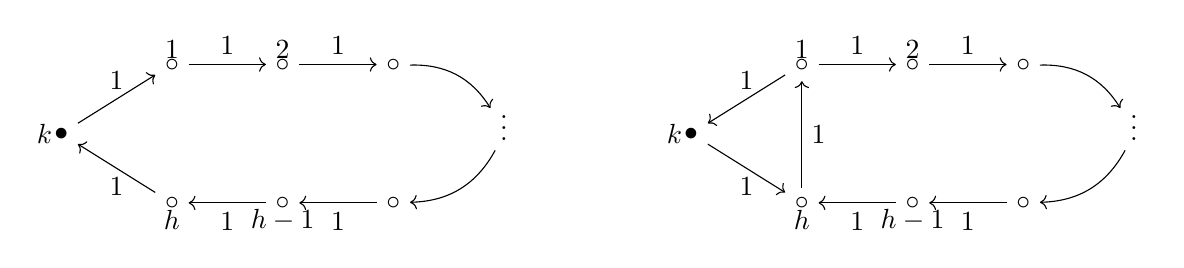
\begin{tikzpicture}[baseline=-0.5ex]
    \matrix[matrix of math nodes,column sep={40pt,between origins},row
    sep={25pt,between origins},nodes={asymmetrical rectangle}] at (0,0)
  {
    & |[name = ul]|\circ& |[name = um]|\circ & |[name = ur]|\circ&\\
    %
    |[name = ml]|\bullet& &&& |[name = mr]|\vdots \\
    %
    & |[name = dl]|\circ& |[name = dm]|\circ & |[name = dr]|\circ&\\
  };
\draw[->]
  (ml) to node[above] {1} (ul)
  ;
  \draw[->]
  (ul) to node[above]{1}(um)
  ;
  \draw[->]
  (um) to node[above]{1}(ur)
  ;
  \draw[->]
  (ur) [bend left] to (mr)
  ;
  \draw[->]
  (mr) [bend left] to (dr)
  ;
  \draw[->]
  (dr) to node[below]{1}(dm)
  ;
  \draw[->]
  (dm) to node[below]{1}(dl)
  ;
  \draw[->]
  (dl) to node[below]{1}(ml)
  ;
    \node at (ml.west){$k$};
    \node at (ul.north){1};
    \node at (um.north){2};
    \node at (dm.south){$h-1$};
    \node at (dl.south){$h$};
    \matrix[matrix of math nodes,column sep={40pt,between origins},row
    sep={25pt,between origins},nodes={asymmetrical rectangle}] at (8,0)
  {
    & |[name = ul]|\circ& |[name = um]|\circ & |[name = ur]|\circ&\\
    %
    |[name = ml]|\bullet& &&& |[name = mr]|\vdots \\
    %
    & |[name = dl]|\circ& |[name = dm]|\circ & |[name = dr]|\circ&\\
  };
\draw[->]
  (ul) to node[above] {1} (ml)
  ;
  \draw[->]
  (ul) to node[above]{1}(um)
  ;
  \draw[->]
  (um) to node[above]{1}(ur)
  ;
  \draw[->]
  (ur) [bend left] to (mr)
  ;
  \draw[->]
  (mr) [bend left] to (dr)
  ;
  \draw[->]
  (dr) to node[below]{1}(dm)
  ;
  \draw[->]
  (dm) to node[below]{1}(dl)
  ;
  \draw[->]
  (ml) to node[below]{1}(dl)
  ;
  \draw[->]
  (dl) to node[right]{1}(ul)
  ;
    \node at (ml.west){$k$};
    \node at (ul.north){1};
    \node at (um.north){2};
    \node at (dm.south){$h-1$};
    \node at (dl.south){$h$};
    \end{tikzpicture}
   
   \item
   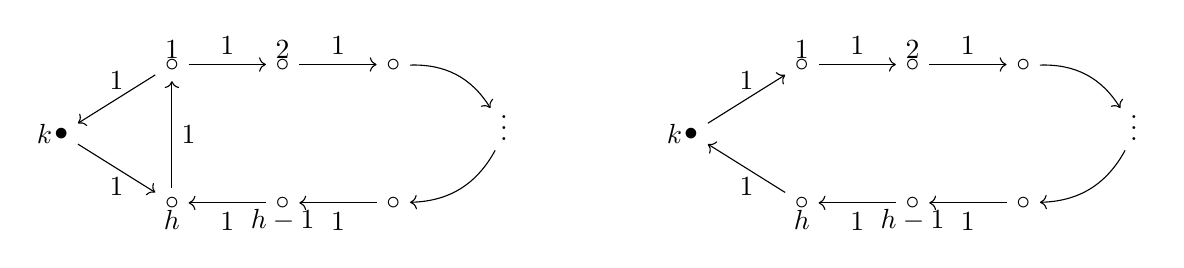
\begin{tikzpicture}[baseline=-0.5ex]
    \matrix[matrix of math nodes,column sep={40pt,between origins},row
    sep={25pt,between origins},nodes={asymmetrical rectangle}] at (8,0)
  {
    & |[name = ul]|\circ& |[name = um]|\circ & |[name = ur]|\circ&\\
    %
    |[name = ml]|\bullet& &&& |[name = mr]|\vdots \\
    %
    & |[name = dl]|\circ& |[name = dm]|\circ & |[name = dr]|\circ&\\
  };
\draw[->]
  (ml) to node[above] {1} (ul)
  ;
  \draw[->]
  (ul) to node[above]{1}(um)
  ;
  \draw[->]
  (um) to node[above]{1}(ur)
  ;
  \draw[->]
  (ur) [bend left] to (mr)
  ;
  \draw[->]
  (mr) [bend left] to (dr)
  ;
  \draw[->]
  (dr) to node[below]{1}(dm)
  ;
  \draw[->]
  (dm) to node[below]{1}(dl)
  ;
  \draw[->]
  (dl) to node[below]{1}(ml)
  ;
    \node at (ml.west){$k$};
    \node at (ul.north){1};
    \node at (um.north){2};
    \node at (dm.south){$h-1$};
    \node at (dl.south){$h$};
    \matrix[matrix of math nodes,column sep={40pt,between origins},row
    sep={25pt,between origins},nodes={asymmetrical rectangle}] at (0,0)
  {
    & |[name = ul]|\circ& |[name = um]|\circ & |[name = ur]|\circ&\\
    %
    |[name = ml]|\bullet& &&& |[name = mr]|\vdots \\
    %
    & |[name = dl]|\circ& |[name = dm]|\circ & |[name = dr]|\circ&\\
  };
\draw[->]
  (ul) to node[above] {1} (ml)
  ;
  \draw[->]
  (ul) to node[above]{1}(um)
  ;
  \draw[->]
  (um) to node[above]{1}(ur)
  ;
  \draw[->]
  (ur) [bend left] to (mr)
  ;
  \draw[->]
  (mr) [bend left] to (dr)
  ;
  \draw[->]
  (dr) to node[below]{1}(dm)
  ;
  \draw[->]
  (dm) to node[below]{1}(dl)
  ;
  \draw[->]
  (ml) to node[below]{1}(dl)
  ;
  \draw[->]
  (dl) to node[right]{1}(ul)
  ;
    \node at (ml.west){$k$};
    \node at (ul.north){1};
    \node at (um.north){2};
    \node at (dm.south){$h-1$};
    \node at (dl.south){$h$};
    \end{tikzpicture}
    
    \item $C$ is an oriented cycle in $\Gamma$ not connected to $k$ and $C'$ is the corresponding cycle in $\Gamma'.$
    
    \item $C$ is an oriented cycle in $\Gamma$ with exactly one vertex in $C$ connected to $k$ by an edge of either weight 1 or 2. Then, $C'$ is the corresponding cycle in $\Gamma'.$  
\end{enumerate}

\end{lem}
\begin{proof}
See \cite[Lemma 2.5]{barot}.
\end{proof}

\section{The Group of a Diagram in an Artin Group}

\begin{defn}
For $\Gamma$ a diagram of finite type, we define the associated Artin Group as follows. The associated artin group $W_\Gamma$ is generated by $s_i,$ where there is one $s_i$ for each vertex $i$ in $\Gamma.$ These generators are subject to the relations
\begin{itemize}
	\item[(R2')] For all $i \neq j,$ we add the relations
	\\
$	\begin{cases}
	s_is_j=s_js_i, &\text{ if there is no edge between $i$ and $j$}\\
	s_is_js_i = s_js_is_j &\text{ if there is an edge of weight 1 between $i$ and $j.$}\\
	s_is_js_is_j = s_js_is_js_i &\text{ if there is an edge of weight 2 between $i$ and $j$.}\\
	s_is_js_is_js_is_j = s_js_is_js_is_js_i &\text{ if there is an edge of weight 3 between $i$ and $j$.}
\end{cases}$
\item[(R3')(a)] For every chordless cycle of the form

\begin{tikzcd}
i_0 \arrow{r} & i_1 \arrow{r} & \cdots \arrow{r} & i_{d-1} \arrow{r} & i_0
\end{tikzcd}

such that all edges have weight 1, for all $i,$ with $0 \leq a \leq d-1,$ we include the relation 
\begin{align*}
	s_{a}s_{a+1}^{-1}s_{a+2}^{-1}\dots s_{a-2}^{-1}s_{a-1}s_{a-2}s_{a-3}\dots s_{a+1} = s_{a+1}^{-1}\dots s_{a-3}^{-1}s_{a-2}^{-1}s_{a-1}s_{a-2}\dots s_{a+1}s_{a}.
\end{align*}
Where subscripts are taken $\pmod d.$ 

\item[(R3')(a)] For every chordless cycle of the form \begin{tikzpicture}[baseline=-0.5ex]
    \matrix[matrix of math nodes,column sep={25pt,between origins},row
    sep={40pt,between origins},nodes={asymmetrical rectangle}] at (6,0)
  {
    && |[name = u]|\bullet& \\
    %
    &|[name=dl]| \circ & &|[name=dr]| \circ \\
  };
\draw[->]
  (u) to node[right] {1} (dr)
  ;
  \draw[->]
  (dl) to node[left]{2}(u)
  ;
  \draw[->]
  (dr) to node[below]{2}(dl)
  ;
  \node [yshift = .4 cm] at (u){i};
    \node [yshift = -.4 cm,xshift = .4 cm] at (dr){j};
    \node [yshift = -.4 cm,xshift = -.4 cm] at (dl){k};
   \end{tikzpicture}
   we include the three relations
   \begin{enumerate}[(1)]
\item $s_{i}s_{j}^{-1}s_{k}s_{j} = s_{j}^{-1}s_{k}s_{j}s_{i}$
\item $s_{j}s_{k}^{-1}s_{i}s_{k} = s_{k}^{-1}s_{i}s_{k}s_{j}$
\item $s_{k}^{-1}s_{i}^{-1}s_{j}s_{i}s_{k}s_{i}^{-1}s_{j}s_{i}s_{k}^{-1}s_{i}^{-1}s_{j}^{-1}s_{i} = e.$
\end{enumerate}
\end{itemize}
\end{defn}

\begin{rem}
Note that if $\Gamma$ is the graph associated to a dynikin diagram, then $W_\Gamma$ as we have defined it is precisely the corresponding Artin group corresponding to that dynkin diagram. This is the case since in this case we have no cycles in $\Gamma,$ and so we only have relation of the form $(R2'),$ which define the Artin Group.
\end{rem}




\section{Additional Pictures}
picure e
\begin{tikzpicture}[baseline=-0.5ex]
\matrix[matrix of math nodes,column sep={40pt,between origins},row
    sep={40pt,between origins},nodes={asymmetrical rectangle}] at (0,0)
  {
    & |[name = ul]|\bullet& |[name = ur]|\circ\\
    %
    &|[name=dl]| \circ &|[name=dr]| \circ \\
  };
\draw[->]
  (ur) to node[above] {1} (ul)
  ;
  \draw[->]
  (ul) to node[left]{2}(dl)
  ;
  \draw[->]
  (dr) to node[below]{1}(dl)
  ;
  \draw[->]
  (ur) to node[right]{2} (dr)
  ;
\draw[->]
  (dl) to node[above]{2} (ur)
  ;
    \node [yshift = .4 cm,xshift = -.4 cm] at (ul){k=1};
   \node  [yshift = .4 cm,xshift = .4 cm] at (ur){2};
    \node [yshift = -.4 cm,xshift = .4 cm] at (dr){3};
    \node [yshift = -.4 cm,xshift = -.4 cm] at (dl){4};
    \matrix[matrix of math nodes,column sep={40pt,between origins},row
    sep={40pt,between origins},nodes={asymmetrical rectangle}] at (6,0)
  {
    & |[name = ul]|\bullet& |[name = ur]|\circ\\
    %
    &|[name=dl]| \circ &|[name=dr]| \circ \\
  };
\draw[->]
  (ul) to node[above] {1} (ur)
  ;
  \draw[->]
  (dl) to node[left]{2}(ul)
  ;
  \draw[->]
  (dr) to node[below]{1}(dl)
  ;
  \draw[->]
  (ur) to node[right]{2} (dr)
  ;
    \node [yshift = .4 cm,xshift = -.4 cm] at (ul){k=1};
   \node  [yshift = .4 cm,xshift = .4 cm] at (ur){2};
    \node [yshift = -.4 cm,xshift = .4 cm] at (dr){3};
    \node [yshift = -.4 cm,xshift = -.4 cm] at (dl){4};
 
   \end{tikzpicture}
Picture g
   \begin{tikzpicture}[baseline=-0.5ex]

    \matrix[matrix of math nodes,column sep={40pt,between origins},row
    sep={40pt,between origins},nodes={asymmetrical rectangle}] at (0,0)
  {
    & |[name = ul]|\bullet& |[name = ur]|\circ\\
    %
    &|[name=dl]| \circ &|[name=dr]| \circ \\
  };
\draw[->]
  (ul) to node[above] {1} (ur)
  ;
  \draw[->]
  (dl) to node[left]{2}(ul)
  ;
  \draw[->]
  (dr) to node[below]{1}(dl)
  ;
  \draw[->]
  (ur) to node[right]{2} (dr)
  ;
    \node [yshift = .4 cm,xshift = -.4 cm] at (ul){k=1};
   \node  [yshift = .4 cm,xshift = .4 cm] at (ur){2};
    \node [yshift = -.4 cm,xshift = .4 cm] at (dr){3};
    \node [yshift = -.4 cm,xshift = -.4 cm] at (dl){4};
 
   \matrix[matrix of math nodes,column sep={40pt,between origins},row
    sep={40pt,between origins},nodes={asymmetrical rectangle}] at (6,0)
  {
    & |[name = ul]|\bullet& |[name = ur]|\circ\\
    %
    &|[name=dl]| \circ &|[name=dr]| \circ \\
  };
\draw[->]
  (ur) to node[above] {1} (ul)
  ;
  \draw[->]
  (ul) to node[left]{2}(dl)
  ;
  \draw[->]
  (dr) to node[below]{1}(dl)
  ;
  \draw[->]
  (ur) to node[right]{2} (dr)
  ;
\draw[->]
  (dl) to node[above]{2} (ur)
  ;
    \node [yshift = .4 cm,xshift = -.4 cm] at (ul){k=1};
   \node  [yshift = .4 cm,xshift = .4 cm] at (ur){2};
    \node [yshift = -.4 cm,xshift = .4 cm] at (dr){3};
    \node [yshift = -.4 cm,xshift = -.4 cm] at (dl){4};
    \end{tikzpicture}
    Picture i
   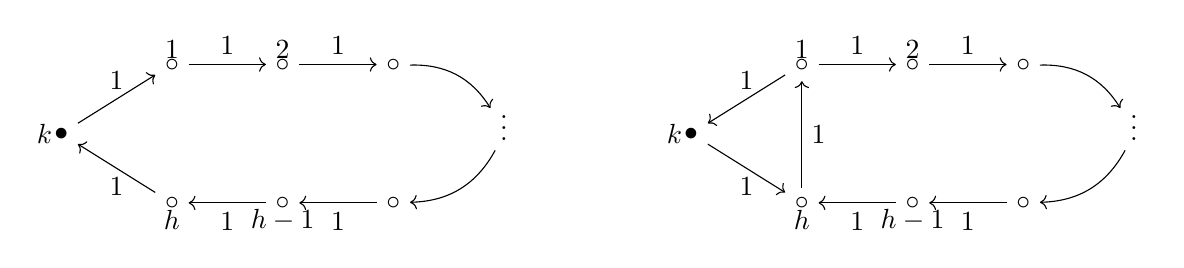
\begin{tikzpicture}[baseline=-0.5ex]
    \matrix[matrix of math nodes,column sep={40pt,between origins},row
    sep={25pt,between origins},nodes={asymmetrical rectangle}] at (0,0)
  {
    & |[name = ul]|\circ& |[name = um]|\circ & |[name = ur]|\circ&\\
    %
    |[name = ml]|\bullet& &&& |[name = mr]|\vdots \\
    %
    & |[name = dl]|\circ& |[name = dm]|\circ & |[name = dr]|\circ&\\
  };
\draw[->]
  (ml) to node[above] {1} (ul)
  ;
  \draw[->]
  (ul) to node[above]{1}(um)
  ;
  \draw[->]
  (um) to node[above]{1}(ur)
  ;
  \draw[->]
  (ur) [bend left] to (mr)
  ;
  \draw[->]
  (mr) [bend left] to (dr)
  ;
  \draw[->]
  (dr) to node[below]{1}(dm)
  ;
  \draw[->]
  (dm) to node[below]{1}(dl)
  ;
  \draw[->]
  (dl) to node[below]{1}(ml)
  ;
    \node at (ml.west){$k$};
    \node at (ul.north){1};
    \node at (um.north){2};
    \node at (dm.south){$h-1$};
    \node at (dl.south){$h$};
    \matrix[matrix of math nodes,column sep={40pt,between origins},row
    sep={25pt,between origins},nodes={asymmetrical rectangle}] at (8,0)
  {
    & |[name = ul]|\circ& |[name = um]|\circ & |[name = ur]|\circ&\\
    %
    |[name = ml]|\bullet& &&& |[name = mr]|\vdots \\
    %
    & |[name = dl]|\circ& |[name = dm]|\circ & |[name = dr]|\circ&\\
  };
\draw[->]
  (ul) to node[above] {1} (ml)
  ;
  \draw[->]
  (ul) to node[above]{1}(um)
  ;
  \draw[->]
  (um) to node[above]{1}(ur)
  ;
  \draw[->]
  (ur) [bend left] to (mr)
  ;
  \draw[->]
  (mr) [bend left] to (dr)
  ;
  \draw[->]
  (dr) to node[below]{1}(dm)
  ;
  \draw[->]
  (dm) to node[below]{1}(dl)
  ;
  \draw[->]
  (ml) to node[below]{1}(dl)
  ;
  \draw[->]
  (dl) to node[right]{1}(ul)
  ;
    \node at (ml.west){$k$};
    \node at (ul.north){1};
    \node at (um.north){2};
    \node at (dm.south){$h-1$};
    \node at (dl.south){$h$};
    \end{tikzpicture}
    
    picture j
    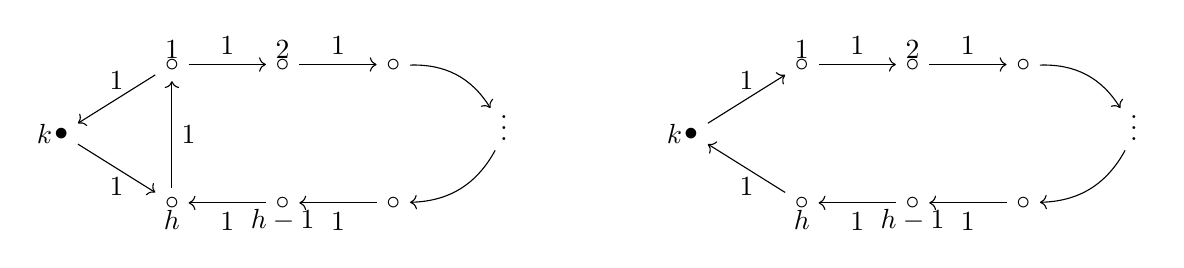
\begin{tikzpicture}[baseline=-0.5ex]
    \matrix[matrix of math nodes,column sep={40pt,between origins},row
    sep={25pt,between origins},nodes={asymmetrical rectangle}] at (8,0)
  {
    & |[name = ul]|\circ& |[name = um]|\circ & |[name = ur]|\circ&\\
    %
    |[name = ml]|\bullet& &&& |[name = mr]|\vdots \\
    %
    & |[name = dl]|\circ& |[name = dm]|\circ & |[name = dr]|\circ&\\
  };
\draw[->]
  (ml) to node[above] {1} (ul)
  ;
  \draw[->]
  (ul) to node[above]{1}(um)
  ;
  \draw[->]
  (um) to node[above]{1}(ur)
  ;
  \draw[->]
  (ur) [bend left] to (mr)
  ;
  \draw[->]
  (mr) [bend left] to (dr)
  ;
  \draw[->]
  (dr) to node[below]{1}(dm)
  ;
  \draw[->]
  (dm) to node[below]{1}(dl)
  ;
  \draw[->]
  (dl) to node[below]{1}(ml)
  ;
    \node at (ml.west){$k$};
    \node at (ul.north){1};
    \node at (um.north){2};
    \node at (dm.south){$h-1$};
    \node at (dl.south){$h$};
    \matrix[matrix of math nodes,column sep={40pt,between origins},row
    sep={25pt,between origins},nodes={asymmetrical rectangle}] at (0,0)
  {
    & |[name = ul]|\circ& |[name = um]|\circ & |[name = ur]|\circ&\\
    %
    |[name = ml]|\bullet& &&& |[name = mr]|\vdots \\
    %
    & |[name = dl]|\circ& |[name = dm]|\circ & |[name = dr]|\circ&\\
  };
\draw[->]
  (ul) to node[above] {1} (ml)
  ;
  \draw[->]
  (ul) to node[above]{1}(um)
  ;
  \draw[->]
  (um) to node[above]{1}(ur)
  ;
  \draw[->]
  (ur) [bend left] to (mr)
  ;
  \draw[->]
  (mr) [bend left] to (dr)
  ;
  \draw[->]
  (dr) to node[below]{1}(dm)
  ;
  \draw[->]
  (dm) to node[below]{1}(dl)
  ;
  \draw[->]
  (ml) to node[below]{1}(dl)
  ;
  \draw[->]
  (dl) to node[right]{1}(ul)
  ;
    \node at (ml.west){$k$};
    \node at (ul.north){1};
    \node at (um.north){2};
    \node at (dm.south){$h-1$};
    \node at (dl.south){$h$};
    \end{tikzpicture}
    
 \begin{thebibliography}{70}

\bibitem{barot}
Barot and Marsh -- CITE THIS CORRECTLY LATER

\end{thebibliography}
\end{document}